% !TeX root = example06.tex
% !TeX program = xelatex
\documentclass{standalone}

\usepackage{amsmath,amsfonts,amssymb,amsthm}
\usepackage{tikz}
\usepackage{pgfplots}
\usepackage{pgfplotstable}
\usepgfplotslibrary{fillbetween}
\usepgfplotslibrary{groupplots}
\usetikzlibrary{arrows}

\usepackage{mathspec}
\setmainfont[BoldFont=Gulliver-Bold,ItalicFont=Gulliver Italic]{Gulliver-Regular}
\setmathrm{Gulliver Italic}
\setmathfont(Digits){Gulliver-Regular}

\setmathfont(Latin)[
BoldFont=Gulliver-Bold,
ItalicFont=Gulliver Italic,
]{Gulliver}

\usepackage{bbm}
\usepackage{bm}
\newcommand{\ve}[1]{\textbf{#1}}

\newcommand{\ba}{\ve{a}}
\newcommand{\bb}{\ve{b}}
\newcommand{\bu}{\ve{u}}
\newcommand{\bv}{\ve{v}}
\newcommand{\br}{\ve{r}}
\newcommand{\bp}{\ve{p}}
\newcommand{\bt}{\ve{t}}
\newcommand{\bn}{\ve{n}}
\newcommand{\bc}{\ve{c}}
\newcommand{\bq}{\ve{q}}
\newcommand{\bff}{\ve{f}}
\newcommand{\bx}{\ve{x}}
\newcommand{\by}{\ve{y}}
\newcommand{\be}{\ve{e}}
\newcommand{\bg}{\ve{g}}
\newcommand{\bs}{\ve{s}}

\newcommand{\bA}{\ve{A}}
\newcommand{\bS}{\ve{S}}
\newcommand{\bB}{\ve{B}}
\newcommand{\bU}{\ve{U}}
\newcommand{\bV}{\ve{V}}
\newcommand{\bQ}{\ve{Q}}
\newcommand{\bP}{\ve{P}}
\newcommand{\bGG}{\ve{G}}
\newcommand{\bRR}{\ve{R}}
\newcommand{\bX}{\ve{X}}
\newcommand{\bC}{\ve{C}}
\newcommand{\bF}{\ve{F}}
\newcommand{\bI}{\ve{I}}

\newcommand{\bLambda}{\boldsymbol{\Lambda}}
\newcommand{\blambda}{\boldsymbol{\lambda}}
\newcommand{\bSigma}{\boldsymbol{\Sigma}}
\newcommand{\bEps}{\boldsymbol{\varepsilon}}
\newcommand{\beps}{\boldsymbol{\varepsilon}}
\newcommand{\heps}{\hat{\varepsilon}}
\newcommand{\bdelta}{\boldsymbol{\delta}}
\newcommand{\vblambda}{\vec{\boldsymbol{\lambda}}}
\newcommand{\vbsigma}{\vec{\boldsymbol{\sigma}}}
\newcommand{\vbEps}{\vec{\boldsymbol{\varepsilon}}}
\newcommand{\vbdelta}{\vec{\boldsymbol{\delta}}}
\newcommand{\eps}{\varepsilon}

\newcommand{\vba}{\vec{\ve{a}}}
\newcommand{\vbu}{\vec{\ve{u}}}
\newcommand{\vbx}{\vec{\ve{x}}}
\newcommand{\vbv}{\vec{\ve{v}}}
\newcommand{\vbs}{\vec{\ve{s}}}
\newcommand{\vq}{\vec{q}}

\newcommand{\hbx}{\hat{\ve{x}}}
\newcommand{\hby}{\hat{\ve{y}}}
\newcommand{\hbz}{\hat{\ve{z}}}

\newcommand{\tx}{\widetilde{\ve{x}}}
\newcommand{\tbB}{\widetilde{\ve{B}}}

\newcommand{\dd}{\text{d}}
\newcommand{\gdot}{\dot\gamma}
\newcommand\Rey{\mbox{\mathrm{Re}}}  % Reynolds number
\newcommand\Ca{\mbox{\mathrm{Ca}}} % Capillary number
\newcommand\Wi{\mathrm{Wi}}  % Weissenberg number
\newcommand\De{\mathrm{De}}  % Deborah number


\textwidth = 6.5 in
\textheight = 8 in

\definecolor{RYB1}{RGB}{207, 37, 37}
\definecolor{RYB2}{RGB}{37, 91, 207}
\definecolor{RYB3}{RGB}{37, 207, 91}
\definecolor{RYB4}{RGB}{163,26,145}
\definecolor{RYB5}{RGB}{253, 180, 98}
\definecolor{RYB6}{RGB}{179, 222, 105}
\definecolor{RYB7}{RGB}{128, 177, 211}

\pgfplotscreateplotcyclelist{newcolors}{
    {RYB1,every mark/.append style={fill=RYB1,mark size={2.5}},mark=*},
    {RYB2,every mark/.append style={fill=RYB2},mark=square*},
    {RYB3,every mark/.append style={fill=RYB3,mark size={3}},mark=triangle*},
    {RYB4,every mark/.append style={fill=RYB4,mark size={3}},mark=diamond*},
    {RYB5,every mark/.append style={fill=RYB5,mark size={3}},mark=pentagon*},
    {RYB6,every mark/.append style={fill=RYB6,mark size={4}},mark=10-pointed star},
    {RYB7,every mark/.append style={fill=RYB7},mark=*},
}

\pgfplotsset{
    standard/.style={
        scale only axis,
        width=0.5\textwidth,
        enlarge x limits=0.05,
        enlarge y limits=0.05,
        max space between ticks=40,
        cycle list name=newcolors,
        every axis/.append style={font=\footnotesize},
        every legend/.append style={font=\footnotesize},
        every node/.append style={font=\footnotesize},
	}
}


\pgfplotsset{/pgfplots/group/every plot/.style={
    title style={at={(0.5,-0.3)},
        xshift=0pt,
        yshift=21pt,
        above}
        }
    }

\begin{document}
\pagestyle{empty}

\begin{tikzpicture}
    \begin{groupplot}[
        group style = {group size = 1 by 2,vertical sep=0.5cm},
        height = 10cm,
        width = 6.5 in]

    \nextgroupplot[standard,
        clip=false,
        title={\footnotesize (a) $\vbv_\eta$},
        axis lines=none,
        xticklabels={,,},
        yticklabels={,,},
        xmin=-1,
        xmax=1,
        ymin=-1,
        ymax=1,
        width=0.33\textwidth,
        height=0.33\textwidth,
        ticks=none,
        ]
        \node[inner sep=0pt] at (axis cs:-0.1,-0.24) {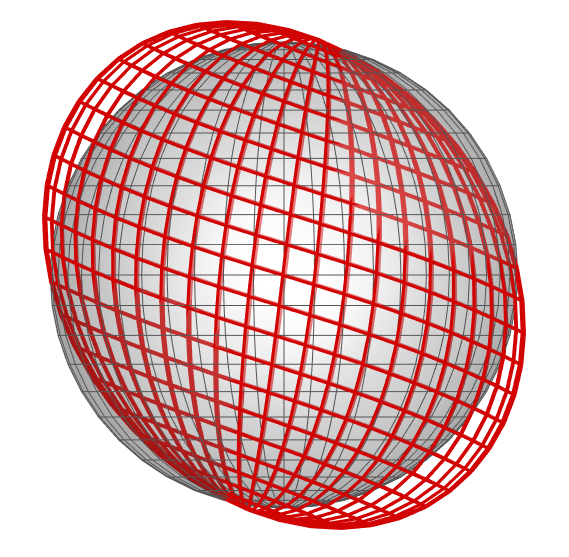
\includegraphics[width=0.21\textwidth]{data/num_abscissa.png}};
        \draw[very thick,latex-latex] (axis cs:-1.2,-0.6) -- (axis cs:-1.2,-1) -- (axis cs:-0.8,-1);
        \node[above] at (axis cs:-1.2,-0.6) {$\hby$};
        \node[right] at (axis cs:-0.8,-1) {$\hbz$};

    \nextgroupplot[standard,
        clip=false,
        title={\footnotesize (b) $\vbv_\Delta$},
        axis lines=none,
        xticklabels={,,},
        yticklabels={,,},
        xmin=-1,
        xmax=1,
        ymin=-1,
        ymax=1,
        width=0.33\textwidth,
        height=0.33\textwidth,
        ticks=none,
        ]
        \node[inner sep=0pt] at (axis cs:-0.1,-0.14) {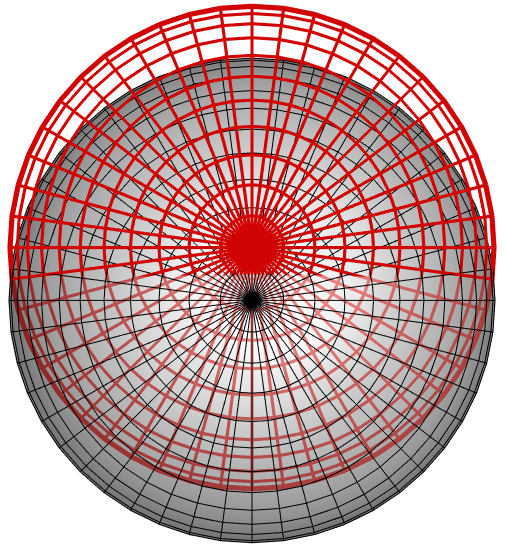
\includegraphics[width=0.19\textwidth]{data/Delta_dist.png}};
        \draw[very thick,latex-latex] (axis cs:-1.2,-0.6) -- (axis cs:-1.2,-1) -- (axis cs:-0.8,-1);
        \node[above] at (axis cs:-1.2,-0.6) {$\hby$};
        \node[right] at (axis cs:-0.8,-1) {$\hbx$};
    \end{groupplot}
\end{tikzpicture} 

\end{document}
